\chapter{Travail et chaleur} 
\section{Définition du concept de travail}
Si un point matériel se déplace le long d'une courbe 1-2 dans 
un champ de force $\vec{F}$, le travail vaudra
\begin{equation}
	W = \int_1^2 \vec{F}.d\vec{x}
\end{equation}
Généralisons pour les systèmes thermodynamiques :\\

\retenir{Un système échange du travail avec le milieu extérieur 
	lorsque l'action du système sur le milieu extérieur peut se 
	réduire au déplacement d'une masse dans le champ de pesanteur.}\ \\

Déplacer un poids n'est pas nécessaire, il faut que l'action 
soit équivalente à celle-ci\footnote{Par convention, un travail 
	est vu comme positif lorsqu'il est reçu par le système.}.\\

\textsc{Exemple.} Comme on peut remplacer le ventilateur par une 
poulie, le moteur effectue bien un travail et interagit avec le 
monde extérieur. 

\begin{center}
	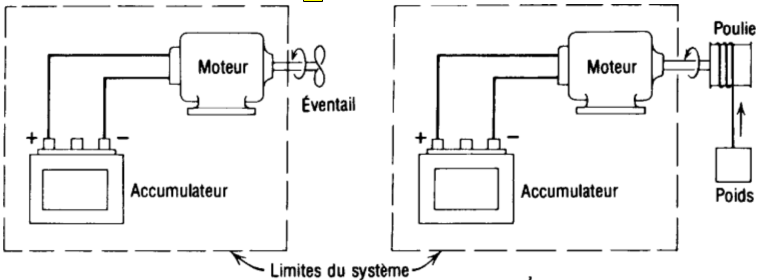
\includegraphics[scale=0.3]{ch4/image1}
	\captionof{figure}{Ceci constitue bien un travail : couple et 
	déplacement angulaire.}
\end{center}

\textsc{Exemple.} Dans ce cas, seul le courant passe la frontière. 
Si par la pensée on connecte les fils à un moteur idéal, la 
présence de courant va générer un travail. Comme il peut être 
rendu équivalent au déplacement d'un poids, il y a donc échange 
de travail.
\begin{center}
	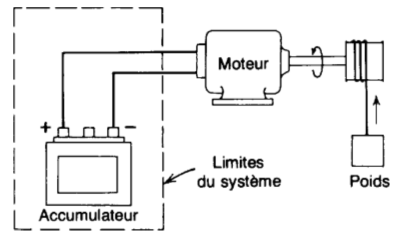
\includegraphics[scale=0.4]{ch4/image2}
	\captionof{figure}{ }
\end{center}

\section{Travail à la frontière mobile d'un système contenant du 
fluide}
\begin{wrapfigure}[7]{r}{4.7cm}
	\vspace{-7mm}
	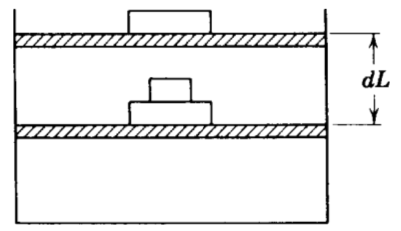
\includegraphics[scale=0.4]{ch4/image3.png}
	\captionof{figure}{ }
\end{wrapfigure}
On a vu le cas d'un arbre tournant, d'un courant : intéressons 
-nous maintenant l'échange de travail à la frontière mobile d'un 
fluide compressible.\\
Si on retire un poids infinitésimal, le piston va monter de $dL$. 
La force exercée par le piston valant $F = p\mathcal{A}$, le 
travail fourni par le système au cours de ce déplacement vaut
\begin{equation}
	\delta W^* = p\mathcal{A}dL = pdV
\end{equation}
En intégrant cette relation, on obtiendra le travail d'une 
transformation quasi-statique. Si l'on connaît la courbe de 
compression dans un diagramme $p-V$, le calcul de $W$ ne sera 
rien d'autre que l'aire sous la courbe entre 1 et 2 qui, dans le cas de la compression, est 
\begin{equation}
	_1W_2 = -\int _1^2 p \, dV
\end{equation}

Attention tout de même :\\
\begin{wrapfigure}[10]{l}{4.7cm}
	\vspace{-7mm}
	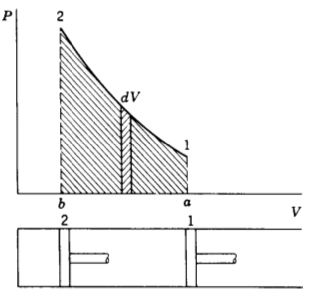
\includegraphics[scale=0.4]{ch4/image4.png}
	\captionof{figure}{Courbe de compression}
\end{wrapfigure}
\vspace{-1cm}
\begin{itemize}
	\item[$\bullet$] Résultat valable ssi la transformation est 
	      quasi-statique !
	\item[$\bullet$] Cette expression ne concerne que cette forme de
	      travail, pas question de l'utiliser avec un ventilateur!
\end{itemize}
La compression de 1 à 2 peut se faire de multiple façon : elle 
dépend des états initial et final mais aussi du chemin 
intermédiaire. Par contre, la variation du volume est indépendante 
du chemin parcouru : $dV$ est une différentielle exacte alors 
que $dW = -pdV$ ne l'est pas $\Longrightarrow$ le volume est 
une variable d'état, pas le travail.\\\\\\


\setcounter{section}{3}
\section{Remarques complémentaires sur le travail}
Le travail échangé ne peut intervenir \textbf{qu'aux} frontières 
du système.\\
\textsc{Exemple.} Considérons la rupture d'une membrane séparant 
el volume d'un gaz du vide. Lorsqu'elle se troue, le gaz se 
répand dans tout le réservoir. Dans la situation ou l'on considère 
le gaz et le vide comme système ($a$), la frontière n'a pas bougée : 
travail nul. 
\begin{center}
	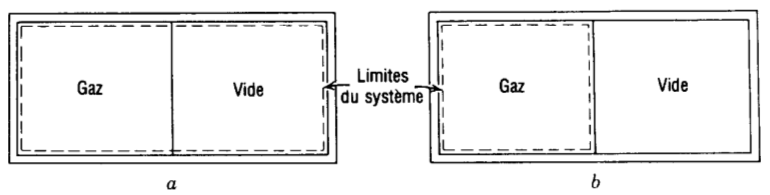
\includegraphics[scale=0.4]{ch4/image5.png}
	\captionof{figure}{ }
\end{center}

Cependant, si l'on considère comme système le gaz seul ($b$),  une variation 
de volume se produit et on a envie de dire $W = -\int_1^2 pdV$ et 
de perdre alors toute crédibilité ! Il ne s'agit \textbf{pas} d'une 
transformation quasi-statique, l'expression ne s'applique pas\footnote{
	En réalité, comme il n'y a pas de résistance aucun travail n'est 
	échangé. Cependant, si l'on place une turbine il sera possible d'obtenir 
un travail sans variation de volume.}.


\section{Définition du concept de chaleur}
En mettant deux corps en contact, ils vont subir une transformation 
pour atteindre l'équilibre thermique : il y a du avoir un \textit{
	transfert d'énergie}. La \textbf{quantité de chaleur} est la forme 
d'énergie transférée durant un tel processus : l'énergie transformée
à la frontière d'un système sous l'effet d'une différence de 
température.\\

Cette définition implique qu'un système contient de l'énergie, mais 
qu'elle ne se manifeste que lors d'un transfert à travers la frontière.\\
On note la chaleur $Q$. Quand $Q=0$, la transformation est dite 
\textit{adiabatique}. Cette chaleur dépend du chemin parcouru, impliquant 
que l'expression ci-dessous n'est pas une différentielle exacte
\begin{equation}
	\ _1Q_2 = \int_1^2 \delta Q
\end{equation}


\section{Comparaison entre chaleur et travail}
Trois similitudes importantes :
\begin{enumerate}
	\item Les deux ne sont mis en évidence que lors d'une transformation. 
	      Un système ne contient ni chaleur, ni travail mais il peut échanger 
	      de l'énergie avec le milieu extérieur sous forme de travail et de chaleur.
	\item Les deux ne sont observés qu'aux frontières.
	\item Les deux dépendent du chemin parcouru.
\end{enumerate}


